\documentclass[12pt]{article}

% Layout.
\usepackage[top=1.2in, bottom=0.75in, left=1in, right=1in, headheight=1.0in, headsep=0pt]{geometry}

% Fonts.
\usepackage{mathptmx}
\usepackage[scaled=0.86]{helvet}
\renewcommand{\emph}[1]{\textsf{\textbf{#1}}}

% TiKZ.
\usepackage{tikz, pgfplots}
\usetikzlibrary{calc}
\pgfplotsset{my style/.append style={axis x line=middle, axis y line=middle, xlabel={$x$}, ylabel={$y$}}}
\pgfplotsset{compat=1.18}

% Misc packages.
\usepackage{amsmath,amssymb,latexsym}
\usepackage{graphicx}
\usepackage{array}
\usepackage{xcolor}
\usepackage{multicol}

% Commands to set various header/footer components.
\makeatletter
\def\doctitle#1{\gdef\@doctitle{#1}}
\doctitle{Use {\tt\textbackslash doctitle\{MY LABEL\}}.}
\def\docdate#1{\gdef\@docdate{#1}}
\docdate{Use {\tt\textbackslash docdate\{MY DATE\}}.}
\def\doccourse#1{\gdef\@doccourse{#1}}
\let\@doccourse\@empty
\def\docscoring#1{\gdef\@docscoring{#1}}
\let\@docscoring\@empty
\def\docversion#1{\gdef\@docversion{#1}}
\let\@docversion\@empty
\makeatother

% Headers and footers layout.
\makeatletter
\usepackage{fancyhdr}
\pagestyle{fancy}
\fancyhf{} % Clears all headers/footers.
\lhead{\emph{\@doctitle\hfill\@docdate} \medskip
\ifnum \value{page} > 1\relax\else\\
\emph{Name: \rule{3.5in}{1pt}\hfill \@docscoring}
\fi}

\rfoot{\emph{\@docversion}}
\lfoot{\emph{\@doccourse}}
\cfoot{\emph{\thepage}}
\renewcommand{\headrulewidth}{0pt}%
\makeatother

% Paragraph spacing
\parindent 0pt
\parskip 6pt plus 1pt

% A problem is a section-like command. Use \problem{5} for a problem worth 5 points.
\newcounter{probcount}
\newcounter{subprobcount}
\setcounter{probcount}{0}

\newcommand{\problem}[1]{%
\par
\addvspace{4pt}%
\setcounter{subprobcount}{0}%
\stepcounter{probcount}%
\makebox[0pt][r]{\emph{\arabic{probcount}.}\hskip1ex}\emph{[#1 points]}\hskip1ex}

\newcommand{\thesubproblem}{\emph{\alph{subprobcount}.}}

% like \problem but with name
\newcommand{\nameprob}[2]{%
\par
\addvspace{4pt}%
\setcounter{subprobcount}{0}%
\stepcounter{probcount}%
\makebox[0pt][r]{\emph{#1.}\hskip1ex}\emph{[#2 points]}\hskip1ex}

% Subproblems are an enumerate-like environment with a consistent
% numbering scheme.  Use \begin{subproblems}\item...\item...\end{subproblems}
\newenvironment{subproblems}{%
\begin{enumerate}%
\setcounter{enumi}{\value{subprobcount}}%
\renewcommand{\theenumi}{\emph{\alph{enumi}}}}%
{\setcounter{subprobcount}{\value{enumi}}\end{enumerate}}

% Blanks for answers in normal and math mode.
\newcommand{\blank}[1]{\rule{#1}{0.75pt}}
\newcommand{\mblank}[1]{\underline{\hspace{#1}}}
\def\emptybox(#1,#2){\framebox{\parbox[c][#2]{#1}{\rule{0pt}{0pt}}}}

% Misc.
\renewcommand{\d}{\displaystyle}
\newcommand{\ds}{\displaystyle}


\doctitle{Math 252: Quiz 2 (corrected)}
\docdate{4 Sept 2025}
\doccourse{}
\docversion{}
\docscoring{\fbox{{\LARGE \strut}\blank{0.8in} / 25}}

\begin{document}
30 minutes maximum.  No aids (book, calculator, etc.) are permitted.  Show all work and use proper notation for full credit.  Answers should be in reasonably-simplified form.  25 points possible.

\begin{enumerate}
% [Like 2.1 \# 2,4,6,8,10] 
\item (9 points) The region $R$, bounded by $y=e^x,$  $y=e^{-x}$ and $x=2$ is sketched below. \\
%%%% GRAPH OF R
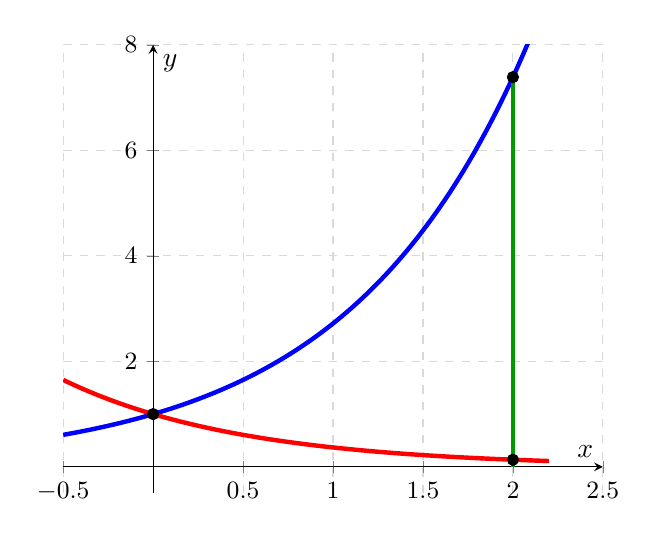
\begin{tikzpicture}
\begin{axis}[
    axis lines = center,
    xlabel = {$x$},
    ylabel = {$y$},
    xmin = -0.5,
    xmax = 2.5,
    ymin = -0.5,
    ymax = 8,
    samples = 100,
    grid = major,
    grid style = {dashed, gray!30},
    tick label style = {font=\small},
]
% Plot the curves
\addplot[ultra thick, blue, domain=-0.5:2.2] {exp(x)};
\addplot[ultra thick, red, domain=-0.5:2.2] {exp(-x)};

% Plot the vertical line x=2
\draw[ultra thick, green!60!black] (axis cs:2,0) -- (axis cs:2,7.389);

% Mark key points
\addplot[only marks, mark=*, mark size=2pt, black] coordinates {(0,1) (2,7.389) (2,0.135)};

\end{axis}
\end{tikzpicture}
	\begin{enumerate}
	\item Label each of the three graphs with the appropriate equation.\\
	
	\item Set up and evaluate an integral to calculate the area of region $R.$ Your answer should be in reasonable simplified form.\\	
	\vfill
	
	\end{enumerate}
%[2.2 \# 68 almost exactly]	
\item (5 points)  Suppose a solid has a base that is the top-half of a circle of radius $a$ and slices perpendicular to the base are squares. The base and a sample rectangle are below. Set up an integral to find its \textbf{volume}. You do not need to evaluate the integral.

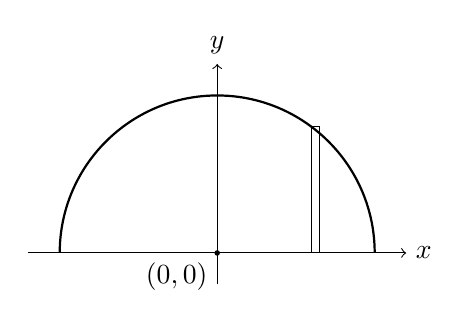
\begin{tikzpicture}[scale=2]
    % Draw coordinate axes
    \draw[->] (-1.2,0) -- (1.2,0) node[right] {$x$};
    \draw[->] (0,-0.2) -- (0,1.2) node[above] {$y$};
    
    % Draw the top half of the unit circle
    \draw[thick] (-1,0) arc (180:0:1);
    
    % Define the width parameter for the rectangle
    % You can change this value to get different rectangle sizes
    \def\a{0.6}
    \def\b{\a+.05}
    
    % Calculate the height of the rectangle
    % For a point at x=a on the unit circle, y = sqrt(1-a^2)
    \pgfmathsetmacro{\h}{sqrt(1-\a*\a)+.003}
    
    % Draw the inscribed rectangle
    \draw[thin] (\a,0) --  (\a,\h) -- (\b,\h) -- (\b,0);
      
    % Mark the center
    \fill (0,0) circle (0.5pt) node[below left] {$(0,0)$};
    
\end{tikzpicture}
\newpage
% [like 2.2 \# 76-98]
\item (11 points) Let $R$ be the region bounded by $y=2x^2$, $y=0,$ and $x=1.$
	\begin{enumerate}
	\item Sketch the region $R$, label the graphs with their equations, and label the points of intersection with their coordinates. \\
	
	\begin{tikzpicture}[scale=.6]
	\draw[ultra thick, ->] (-2,0) -- (6,0);
	\draw[ultra thick, ->] (0,-2) -- (0,6);
	\draw[thick] (3, -.1) -- (3, .1);
	\node at (3,-.5){$1$};
	\node at (6,-.4){$x$};
	\node at (-.4,6){$y$};
	\end{tikzpicture}
	
	\item Use disks to find the volume of the solid obtained by rotating $R$ about the $x$-axis. 
		\vfill
	\item Use washers to find the volume of the solid obtained by rotating $R$ about the $y$-axis. \	\vfill
	\end{enumerate}
\end{enumerate}
\end{document}

